\chapter{Literature Review}
\renewcommand{\baselinestretch}{\mystretch}
\label{chap:Litera}
%\setlength{\parindent}{0pt}

\section{3D printing system}

\PARstart{3}{D} printing is an old but energetic technology, which is also named as additive manufacturing(AM). This idea was put into practice for rapid prototyping at the end of the 1980s and the beginning of the 1990s  \cite{long20173d} . In recent years, its development has attracted extensive interest from people in different fields. 3D printing has become one of the most popular manufacturing techniques in the industry. It has influenced mechanical manufacturing, architecture and medical fields. \\
\\
In the last decade, the cost of 3D printing system has dropped dramatically. In fact, 3D printing is getting into common usages and imaginations, which even be facilitated in families and companies. People could print their own designs with a 3D printer. More and more 3D printers have been designed  with a low price and the simple operations. A variety of raw materials have been investigated in 3D printing field. It is no surprise that 3D printing has been targeted as a reliable production technique. There are three groups of systems for additive manufacturing, which are recognised as liquid-based systems, solid-based systems and powder-based systems. The classification of 3D printing is organised in Figure \ref{Fig:classification}. In below, the most popular technique from each group will be introduced. 

\begin{figure}[htbp]
  \centering
  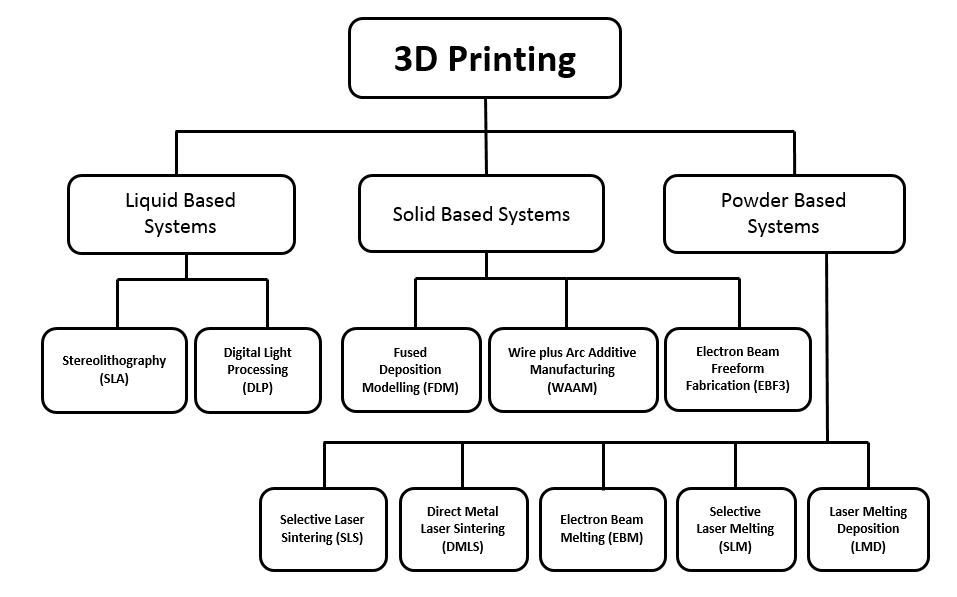
\includegraphics[scale=0.5]{Figs//3D_print_classification.PNG}
  \caption[The classification of 3D printing techniques]{\footnotesize The classification of 3D printing techniques.}
  \label{Fig:classification}
\end{figure}


\subsection{Stereolithography apparatus}

In history, Stereolithography apparatus (SLA) is the earliest 3D printing technology which was invented by Charles (Chuck) Hull in 1986. From then, SLA opened the door to commercialize the Rapid Prototyping (RP) system \cite{zhou2000parametric}. Stereolithography is based on laser technology and it belongs to the liquid-based system group. In the SLA 3D printing system as Figure \ref{Fig:SLA} presents, a UV laser scans the surface of the liquid resin then solidifies the layer selectively. The liquid material is contained in the tank. The platform would be moved down after one layer is scanned. A new layer of liquid resin will be hardened. The repetition of layer solidification could obtain an entire 3D object. Also,  a computer is embedded in the machine which could control the platform and the laser by reading a STL file. \\
\\
Stereolithography paves a way to create a considerably accurate 3D build with short time and respectively low cost. Therefore, SLA has gained wide acceptance in different fields, such as jewellery models \cite{leong1998abrasive} , replicas of heart for simulation of surgical operation \cite{shiraishi2014development}, etc.\\
\\
In terms of the raw materials for SLA, resin-based photopolymers are the basic idea. These liquid materials could react by solidifying when they are cured by a high-powered laser or light source. In practice, the energy from the laser is significant in SLA printing and it is affected by several elements, such as the scan speed, the cured time, the light and the material \cite{chia2015recent}. The limitation of available photopolymers becomes the main weakness of this technology \cite{wang2016stereolithographic}. However, there is a definite possibility that a wide variety materials are combined with photopolymers as the candidates for SLA technique, including short fibre \cite{yunus2017short}, ZrO2-reinforced Al2O3 components \cite{licciulli2005laser} and epoxy, diethylene triamine and silica powder \cite{scarparo1996mechanisms}. 

\begin{figure}[t]
  \centering
  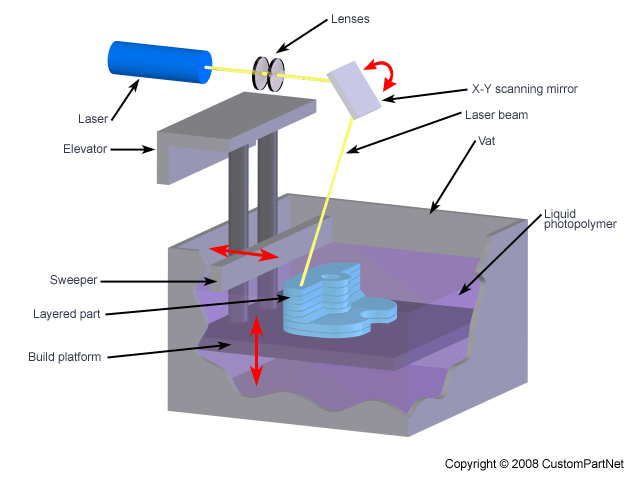
\includegraphics[scale=0.5]{Figs//SLA_PROCESS.png}
  \caption[SLA process]{\footnotesize SLA process.}
  \label{Fig:SLA}
\end{figure}

\subsection{Fused deposition modelling}

Fused Deposition Modelling (FDM) rapid prototyping system was firstly built by Scott Crump in 1988 \cite{hashmi2014comprehensive}, which is also known as Fused Filament Modelling (FFM). It is a considerably popular and low-cost technology for functional manufacturing. FDM system relies on filament extrusion \cite{carneiro2015fused}. In general, FDM system controls the nozzle head to produce all prints and the feature size of the production is limited by the die size in nozzle correspondingly. The FDM system in Figure \ref{Fig:FDM} heats and melts thermoplastic material by a nozzle head. And the concept of selective deposition is also applied \cite{dul2016fused}. The filament is fed by the motor and it is molten through the heater inside. The liquefier moves through the nozzle die and solidifies to the thin filament \cite{singh2014process}. The nozzle head moves horizontally and deposits material according to the design for current layer. The build plate moves down vertically when the printer finished one layer. After fabrication of each layer, the 3D model is complete without any hardening \cite{jin2015quantitative}.\\
\\
In this technique, there are lots of elements or parameters could influence the quality of products such as surface roughness. In terms of the properties of the material, the extruding temperature is decided by their glass transition temperature. The humidity, density and adhesion property of the material also cannot be neglected \cite{chohan2016mathematical}\cite{costa2017estimation}. As for other settings in the machine, the orientation, layer thickness, air gap, raster angle and width should be taken into consideration \cite{rao2016optimization}. Meanwhile, there are several build parameters which affect production accuracy and manufacture efficiency as well \cite{griffiths2016effect}\cite{boschetto2016design}.
 
\begin{figure}[htbp]
  \centering
  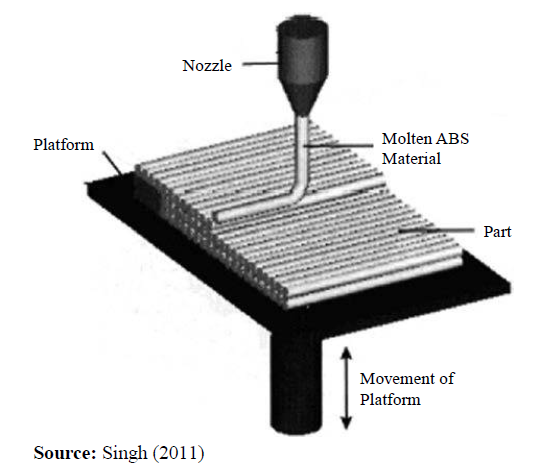
\includegraphics[scale=0.6]{Figs//FDM_process.PNG}
  \caption[FDM process]{\footnotesize FDM process.}
  \label{Fig:FDM}
\end{figure}

\subsection{Selective laser sintering}

Selective laser sintering uses layer printing to build a 3D model\cite{hashmi2014comprehensive}. It selectively fuses small particles of plastic, metal, ceramic or glass powders by a high power laser beam\cite{jiang2013study}. As can be seen in Figure \ref{Fig:SLS}, the materials for this process are powders which is placed in the container initially and spread on the building platform later. The building platform is lowered down every single layer finishes scanning by the laser according to its geometrical design\cite{shahzad2013additive}\cite{shahzad2014additive}. This procedure is repeated until the print is complete\cite{ganeriwala2014multiphysics}. \\
\\
This technique is without material moulding. Parts possess high mechanical properties\cite{zhu2015investigation}. This process is quite fast for printing functional, durable parts. It enables complex parts with interior components and without rapping the material inside and altering the surface from support removal. What’s more, there are vast variety of materials which could be applied for this technique, such as polypropylene (PP) powder \cite{zhu2015investigation}, PA12 and PEKK \cite{peyre2015experimental}, nanoparticle agglomeration\cite{yuksel2016modeling}. In fact, SLS regards Nylon based materials as the candidate materials. The weakness of this technique is the surface porosity of SLS printed parts. 

\begin{figure}[htbp]
  \centering
  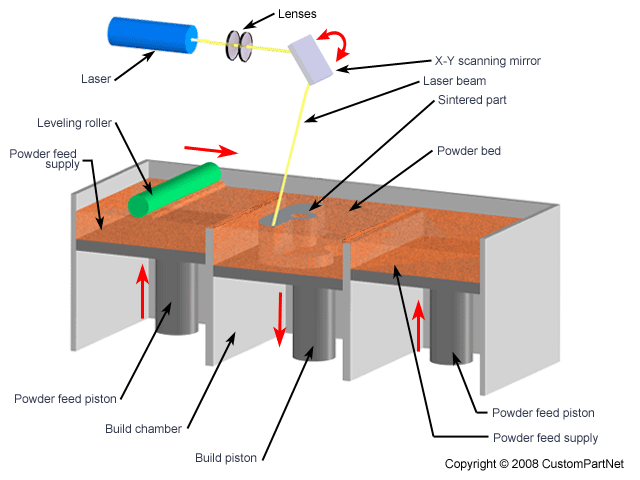
\includegraphics[scale=0.5]{Figs//SLS_process.png}
  \caption[SLS process]{\footnotesize SLS process.}
  \label{Fig:SLS}
\end{figure}

\section{3D printing materials}

The remarkable development of 3D printing technology provides insights into usage of various plastic polymers. The usage of virgin material is no more common since its high cost and time-consuming. Otherwise, people utilise the basic 3D printing materials as the base to combine with metal oxides, short fibres and other polymers as a new material to obtain some special properties \cite{torrado2015characterizing}. Since there are lots of durable and compatible plastic, it could be renewed and reused after adding the virgin material. \\
 \\
In fact, there are several popular thermoplastics for industrial manufacturing as well as personal work since they are low-cost and compatible. According to their different physical and chemical properties, they are applied for additive manufacturing with different techniques or settings. In figure \ref{Fig:material-per-stampanti}, it is clear that the products printed with PLA, ABS and Nylon are distinct. Furthermore, the details of these three materials would be explained below.
\\
\begin{figure}[htbp]
  \centering
  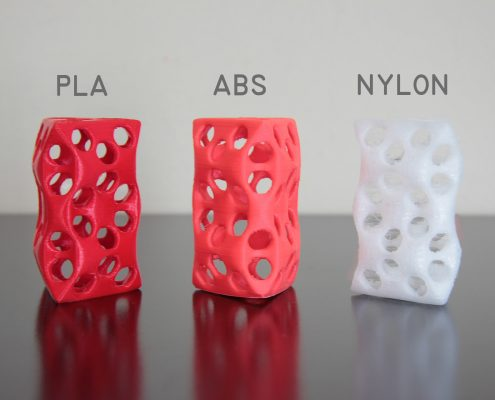
\includegraphics[scale=0.5]{Figs//materiali-per-stampanti-3D.jpg}
  \caption[3D prints made of different materials]{\footnotesize 3D prints made of different materials.}
  \label{Fig:material-per-stampanti}
\end{figure}

\subsection{Acrylonitrile butadiene styrene}

Acrylonitrile butadiene styrene (ABS) is a kind of thermoplastics polymer which plays a significant role in FDM rapid prototyping system. As the name suggests, ABS is composed of polymerising styrene and acrylonitrile in the presence of polybutadiene. ABS has no real melting point and its glass transition temperature is about 105 $^{\circ}$C (221 $^{\circ}$F)\cite{rutkowski1986acrylonitrile}.  ABS could be recycled and it is environmentally friendly. It is usually utilised between 20 and 80 $^{\circ}$C (−4 and 176 $^{\circ}$F) since it remains a relatively stable at a low temperature.\\
\\
Based on its mechanical properties, its impact resistance and high tensile strength enable it to build durable products, like the famous Lego bricks and other outer bodies of office facilitates. Its electrical property paves a new way to produce light and cost-effective electrical components, which work well over a wide range of frequencies. It is not surprised that 3D printed electromagnetic structures such as antenna\cite{mirzaee2015developing} and insulator\cite{mehmood2017performance} are made by ABS materials. ABS has attracted lots of interest from people since they could DO-IT-YOURSELF (DIY) with ABS filament at home. It is easy to design or download models from the Internet and print them to get some lovely products as Figure \ref{Fig:ABS product} shows.

\begin{figure}[htbp]
  \centering
  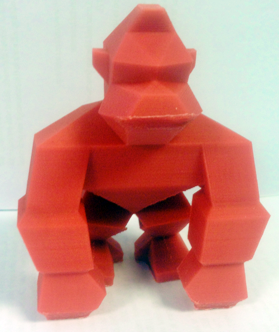
\includegraphics[scale=0.9]{Figs//ABS_product.png}
  \caption[3D-printed King Kong made of ABS]{\footnotesize 3D-printed King Kong made of ABS.}
  \label{Fig:ABS product}
\end{figure}

\subsection{Polylactic acid}

Polylactic acid (PLA) is similar to ABS for its renewable property. In particular, PLA belongs to bioplastic due to its biodegradable and bioactive properties. There are several types of PLA including PLLA (Poly-L-lactic Acid), PDLA (Poly-D-lactic Acid) and PDLLA (Poly-DL-lactic Acid) which are all derived from the renewable resource called lactic acid\cite{sodergaard2010industrial}. What should be concerned is the glass transition temperature of PLLA is between 60 and 65 $^{\circ}$C and its melting point is 157 - 170 $^{\circ}$C. It means PLA cannot be applied at a high temperature. In additive manufacturing, the typical injection moulding temperature of PLLA is about 178 - 240 $^{\circ}$C.\\
\\
More importantly, PLA is extremely robust in the normal application. Compared with ABS, PLA is a little bit less toxic and non-petroleum. And it is widely utilised in food packaging\cite{marra2017assessment} and medical implants\cite{bergstrom2016overview}. As a kind of dielectric material, PLA is also taken into use for antenna production\cite{mirzaee2016high}. PLA is also compatible and there are several PLA blends, such as Aluminum PLA as Figure \ref{Fig:PLA product} below .

\begin{figure}[htbp]
  \centering
 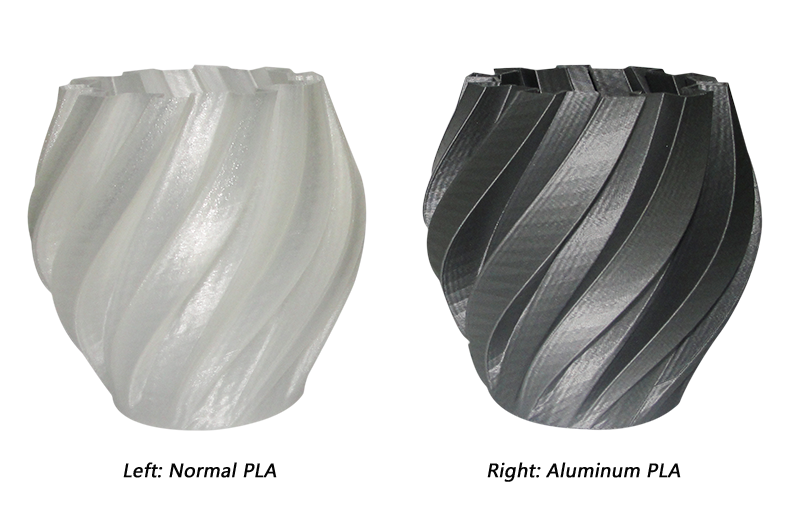
\includegraphics[scale=0.4]{Figs//aluminum-PLA_2.png}
  \caption[Pure PLA and Aluminum PLA products]{\footnotesize Pure PLA and Aluminum PLA products.}
  \label{Fig:PLA product}
\end{figure}


\subsection{Polyamide}

Nylon stands for a family of synthetic polymers. It was first invented by Dr. Wallace Hume Carothers as an ideal synthetic fibre in 1927 \cite{doi:10.1021/ed021p88}. With the development of Nylon production, it has become a kind of smooth thermoplastic material that could be fabricated into shapes, fibres or films. Pure Nylon has the critical problem about storage as it always absorbs moisture from the air and it is difficult to dry it. Therefore, people blend nylon with other fibres or polymers creatively to get an exceptionally durable Nylon blends.\\
\\
 In 3D printing, Nylon is a considerably attractive material for SLS technique \cite{shaw2016investigation}. In addition, there exists Nylon filament which is a candidate material for FDM system. Nylon filament is an incredibly durable, versatile and strong AM material. It is flexible with very high adhesion. Its low friction coefficient and high melting temperature are beneficial for FDM technique. In this case, application of Nylon varies from Artificial Muscles\cite{arjun2016design}, Nylon tube \cite{webb2006integration} to polyamide lens \cite{bunea2014investigation}.
 
\section{3D manufacture in space}

As it is mentioned before, there is an urgent requirement to apply 3D printing in space for long-term research. Actually, it has been verified that FDM technique is suitable and safe in the micro-gravity environment of the International Space Station\cite{fateriadditive}. Moreover, scientists also use 3D printing in aerospace by using a special Zero-Gravity 3D printer \cite{joshi20153d}. \\
\\
In fact, there are several groups researching on the In-situ resource utilisation for sustainable development of 3D printing in space \cite{kading2015utilizing}. In recent years, Lunar and Martian regolith in space are not mysterious for human beings anymore. Based on their multi-component ceramic property, there is no doubt to utilise them in the powder based system that is Selective Laser Melting (SLM) system \cite{goulas20163d}. However, it has been demonstrated that only lunar dust is a suitable material for this system while Martian dust is not \cite{goulas2017assessing}.  Additionally, there is a weakness of this technique with Lunar dust that the geometrical accuracy of the product should be improved \cite{fateriadditive}. And the vacuum environment is also a challenge for SLM technique.\\
\\ 
According to these studies, utilisation of Lunar and Martian regolith for FDM technique has emerged as an interesting topic. The combination of lunar/martian regolith and bio-derived polymers was successfully utilised for 3D printing \cite{jakus2017robust} as Figure \ref{Fig:lUNAR PRITNS} presents. Therefore, there is a strong possibility to produce other blends by mixing these two types of regolith with other printable polymers\cite{ray2010jsc}. 
 \\
 
\begin{figure}[htbp]
  \centering
  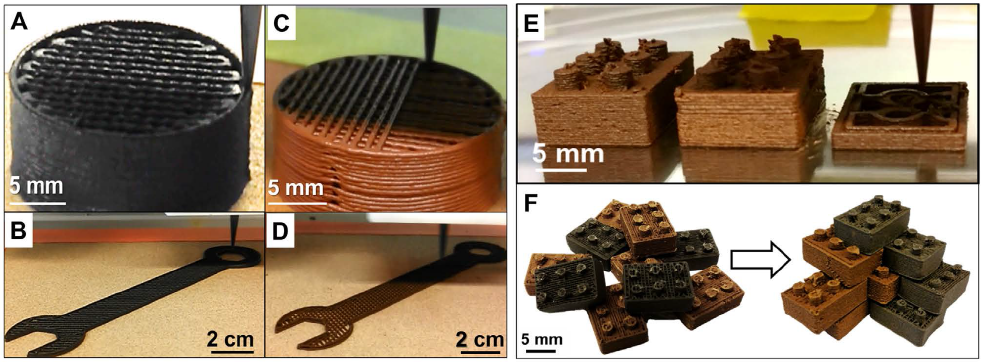
\includegraphics[scale=0.5]{Figs//LUNAR_dust_prints.PNG}
  \caption[3D-printed products made of Lunar/Mars dust]{\footnotesize 3D-printed products made of lunar dust(A,B), martian dust (C,D,E) and both (F) inks copyright @ 2017Robust. }
  \label{Fig:lUNAR PRITNS}
\end{figure}

